%!TEX root = ../../architekturdokumentation.tex
\chapter{Logische Architektur}
\section{3-Tier-Architektur}
	Um eine möglichst hohe Abstraktion unseres Codes zu erhalten, haben wir uns für eine 3-Tier-Architektur entschieden, die unsere Applikation in die drei Schichten Web, Service und DataAccesLayer (Dal) unterteilt. Alle Datenbankspezifischen Operationen sollen im DAL vorgenommen werden. Die Zugriffe auf externe Schnittstellen über den Service-Layer. Alle Zugriffe aus dem Web sollen über die Web-Layer behandelt werden. 
    \begin{figure}[h]
  		\vspace{-5pt}
    	\centering
		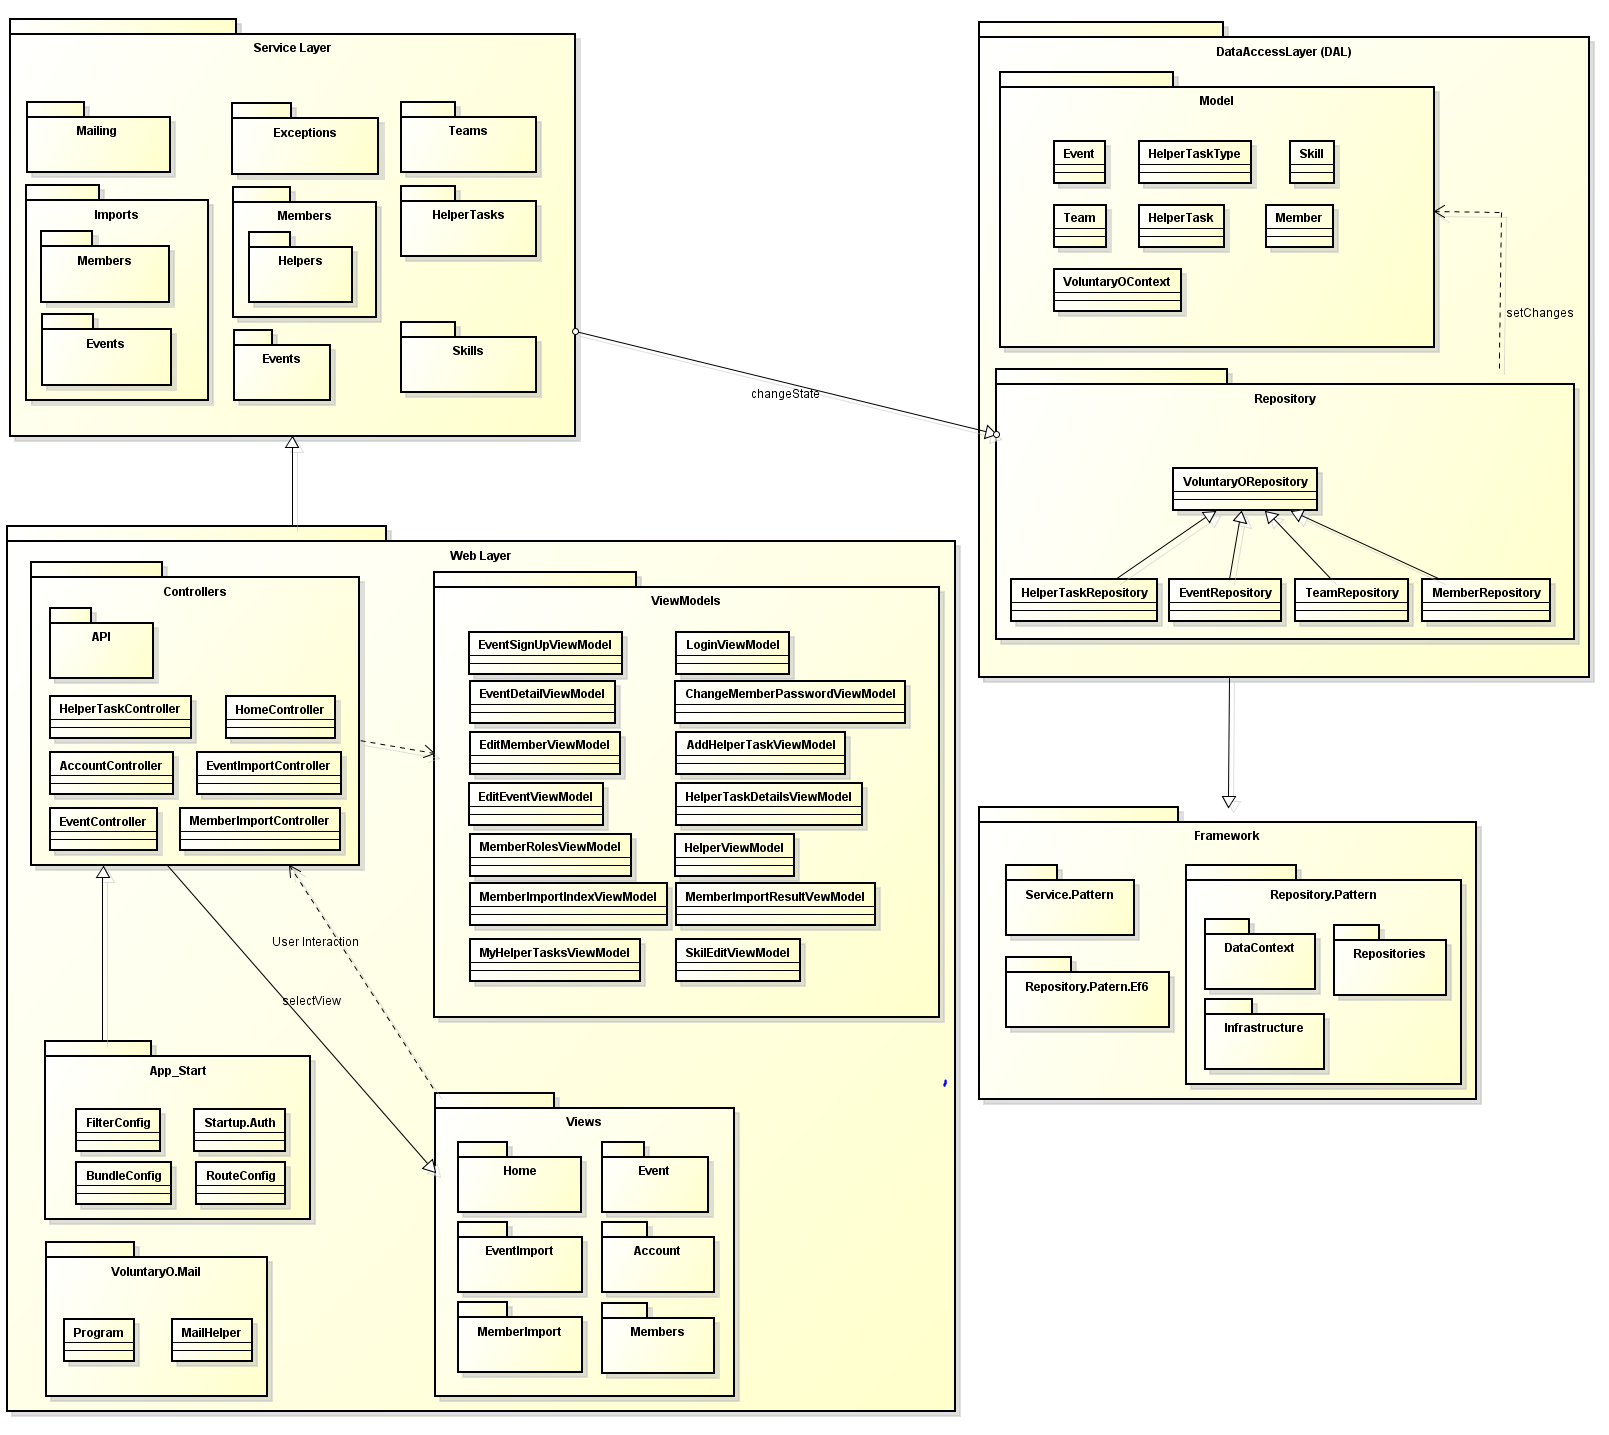
\includegraphics[width=\textwidth]{content/architekturdokumentation/images/LogischeArchitektur.png}
  		\vspace{-20pt}
    	\caption{Logische Architektur}
	\end{figure}

\newpage
\section{VoluntaryO.Dal (Data Access Layer)}
    \begin{figure}[h]
  		\vspace{-5pt}
    	\centering
    	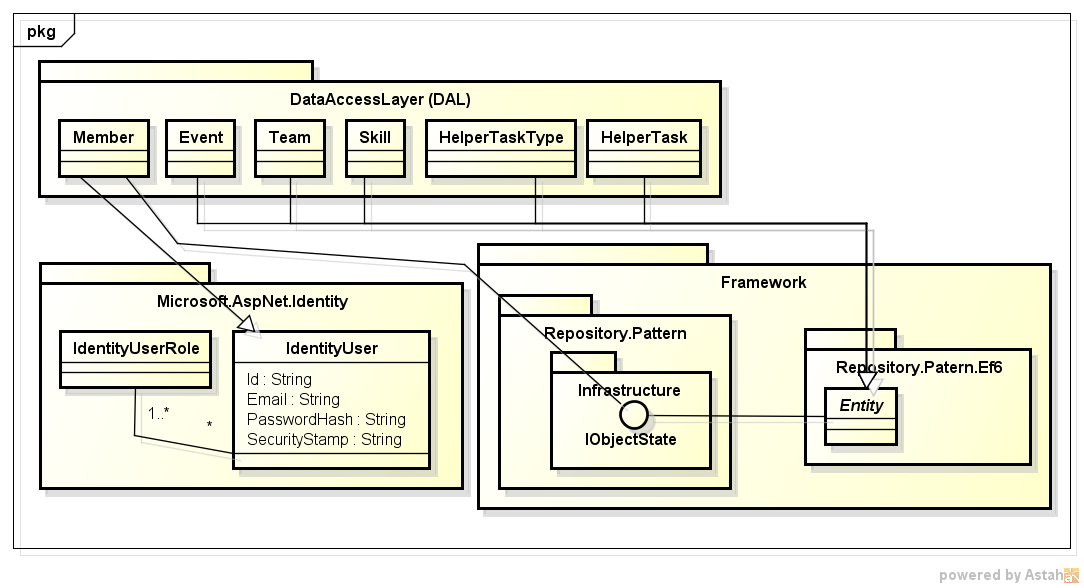
\includegraphics[width=0.7\textwidth]{content/architekturdokumentation/images/VoluntaryO_Dal_Overview.png}
  		\vspace{-20pt}
    	\caption{Klassen in VoluntaryO.Dal}
	\end{figure}
	Jede Model-Klasse implementiert die Schnittstelle \textit{IObjectState}, resp. leitet von der abstrakten Klasse \textit{Entity} ab. Die Verwendung von ASP.NET Identity ist im Kapitel VoluntaryO.Web näher beschrieben.
	
	\subsection{Vergleich für Objekte}
		Einzig für die Member-Klasse wurde die Vergleichsmethode (Equals) überschrieben. Folgende Attribute der Klasse sind relevant:
		\\\begin{itemize}
			\item \textit{UserName}
			\item \textit{Firstname}
			\item \textit{Lastname}
			\item \textit{Birthdate}
		\end{itemize}
		Der Vergleich wurde nur für die Mitgliedsimport-Funktion überschrieben. Für die übrigen Model-Klassen wird die standard Vergleichsmethode beibehalten (Vergleich der Referenz bei Referenztypen).

	\subsection{Repository / Unit of Work Pattern}
		Durch die Verwendung des \href{https://genericunitofworkandrepositories.codeplex.com/}{\textit{Generic Unit of Work \& Repositories Framework}} (in "'Framework"' abgelegt) ergeben sich folgende Vorteile:
		\\\begin{itemize}	
			\item Austauschbarkeit ORM
			\item Testbarkeit
			\item Jeder Request hat eigene Unit of Work (siehe später Dependecy Injection)
			\item Reduktion der Datenbankabfragen, da nur noch über Unit of Work commited wird
			\item Generische Abfragen von Entitäten
		\end{itemize}
		Folgende Konventionen ergeben sich aus für das Projekt:
		\\\begin{itemize}
			\item Jede Entität implementiert \textit{IObjectState}
			\item Repository kann über \textit{partial Classes} erweitern werden
			\item Oder Repository Klassen implementieren \textit{IRepository} und erben von \textit{Repository}
		\end{itemize}

	\subsubsection{Konventionen für eigene Repository Erweiterungen}
		\begin{itemize}
			\item Objekt(-e) abrufen/suchen \textit{Find*}
			\item Objekt(-e) einfügen \textit{Insert*}
			\item Objekt ändern \textit{Update*}
			\item Objekt hinzufügen \textit{Delete*}
			\item Zuweisung zweier Objekte hinzufügen \textit{Assign*}
			\item Zuweisung zweier Objekte entfernen \textit{Unassign*}
		\end{itemize}

	\subsection{Unit Tests mit Effort}
		\href{https://effort.codeplex.com/}{\textit{Effort}} ist ein ADO.Net Provider und erstellt jeweils eine In-Memory Datenbank für das EF. Die temporäre Datenbank ermöglicht uns ein Testen des Codes, ohne Datenbankzugriffe zu mocken.
		\begin{lstlisting}[language=CSharp, caption=Verwendung Effort für Unit Tests in EffortTest.cs, label=lst:effortunittest, firstnumber=1]
			DbConnection Connection = DbConnectionFactory.CreateTransient();
			VoluntaryoContext VoluntaryoContext = new VoluntaryoContext(_Connection);
	    \end{lstlisting}
	    Den einzelnen Unit Tests steht so eine saubere und testbare Datenbank zur Verfügung. Jeder UnitTest erbt von der Abstrakten Klasse \textit{EffortTest}.

	\subsection{Relationales Modell}
	    \begin{figure}[h]
	  		\vspace{-5pt}
	    	\centering
	    	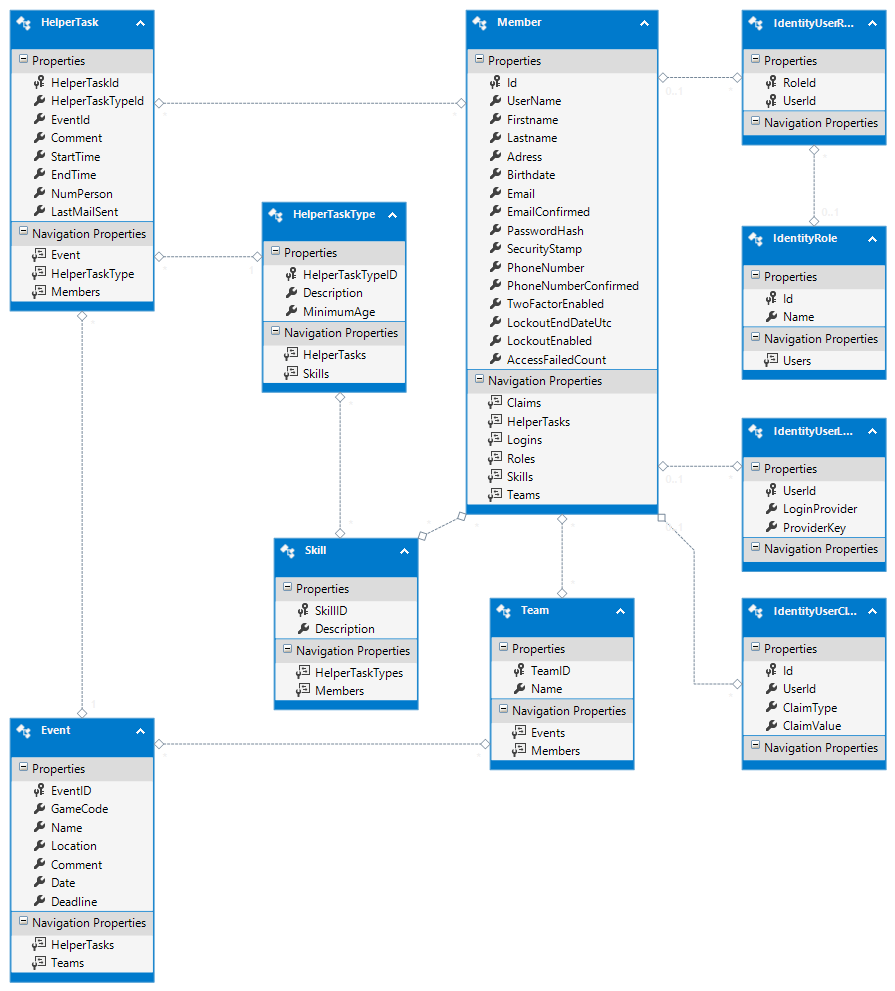
\includegraphics[width=0.7\textwidth]{content/architekturdokumentation/images/edmx.png}
	  		\vspace{-20pt}
	    	\caption{Relationales Modell für VoluntaryO.Dal}
		\end{figure}
		\subsubsection{Mapping}
			Das Mapping wird mit dem \textit{modelBuilder} des EF gesteuert. Bspw.
			\begin{lstlisting}[language=CSharp, caption=Mapping in VoluntaryoContext.cs, label=lst:mappingcontextcs, firstnumber=1]
	// TeamEventMapping
	modelBuilder.Entity<Team>()
	    .HasMany(t => t.Events)
	    .WithMany(e => e.Teams)
	    .Map(mc =>
	    {
	        mc.MapLeftKey("TeamID");
	        mc.MapRightKey("EventID");
	        mc.ToTable("TeamEventMappings");
	    });
		    \end{lstlisting}

\newpage
\section{VoluntaryO.Service}
	Dieses Subprojekt dient als Abstraktionsschicht zwischen den Packages aus dem DAL und deren Verwendung im Web Layer und enthält die eigentliche Business-Logik. Dadurch wird die Logik in den Actions der Controller reduziert und eine höhere Kohäsion erreicht. Die Aufteilung  von Namespaces und Ordner wurde aufgrund der Zugehörigkeit zu den Entitätsklassen im Domainmodell gewählt. Aufgabenspezifische Service-Komponenten wurden ebenfalls in der obersten Hierarchiestufe des Service-Projekts in einem separaten Ordner untergebracht.
	
	\begin{figure}[H]
	    	\centering
	    	 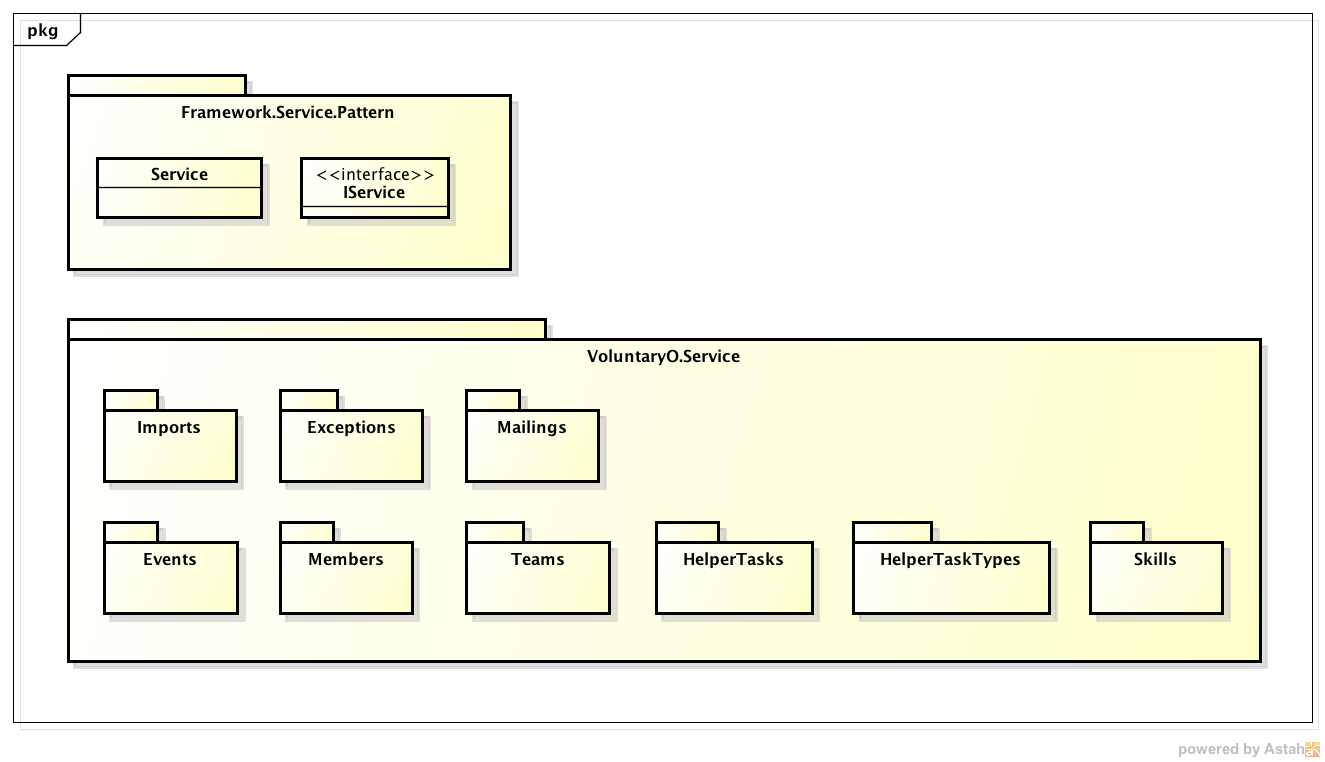
\includegraphics[width=0.9\textwidth]{content/architekturdokumentation/images/Service_Overview.png}
	  		\vspace{-25pt}
			\caption{Packageübersicht des Service-Layers und Service Pattern}
	\end{figure}
	
	\subsection{Verwendung der Service-Klassen}
	Für jedes Repository existiert eine zugehörige Service-Klasse, welche das \textit{IService} Interface implementiert. Dadurch wird die Kopplung zwischen Respositories und Controllern reduziert und eine einheitliche Schnittstelle zur Business-Logik geschaffen:
	
	\begin{figure}[H]
	    	\centering
	    	 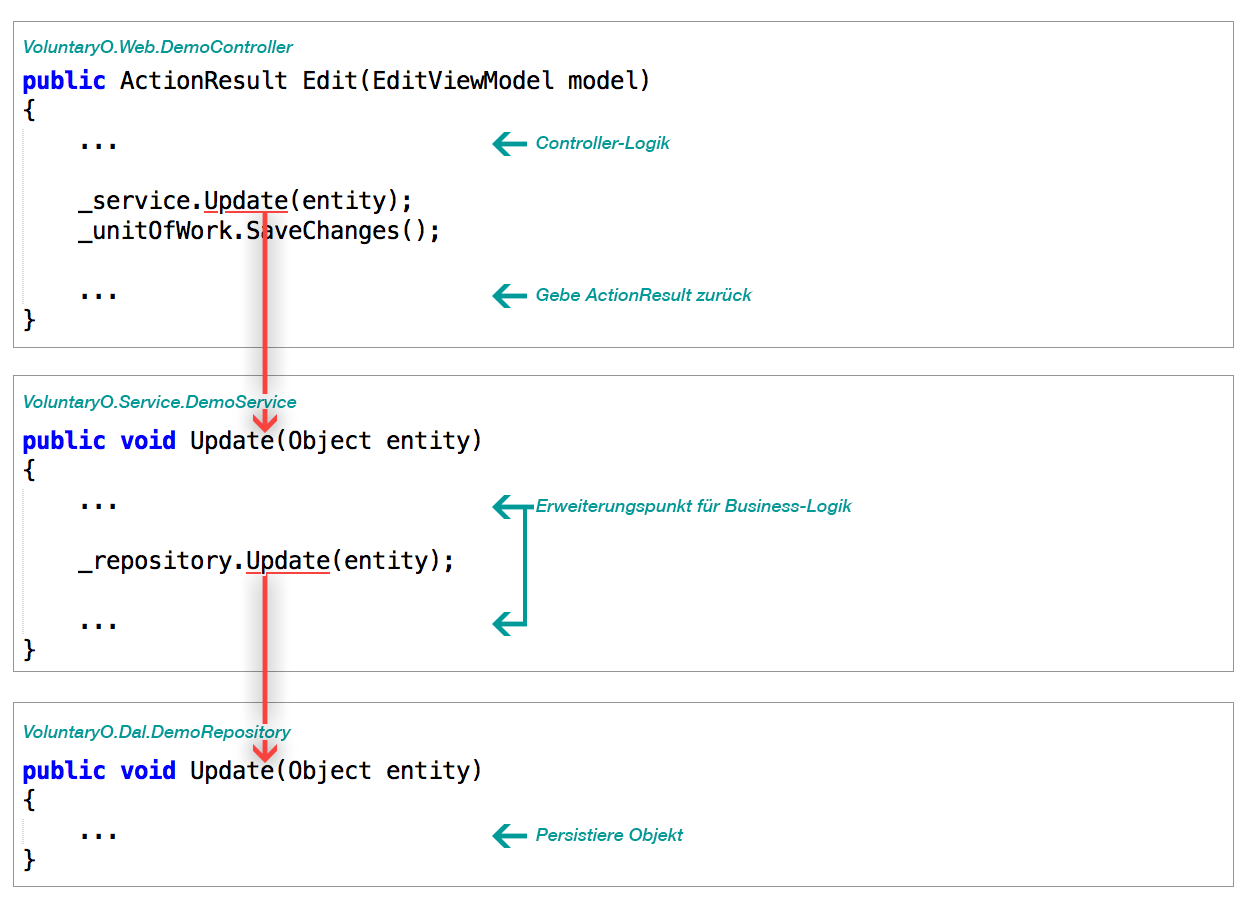
\includegraphics[width=0.9\textwidth]{content/architekturdokumentation/images/Service_Framework_Code.png}
	  		\vspace{-15pt}
			\caption{Aufrufhierarchie über Layers anhand eines Beispiels}
	\end{figure}
	
	\subsection{Aufbau der Service-Klassen}
	Die Vererbungshierarchie aller Service-Klassen (Ausnahme: MailingService) folgt immer dem selben Schema. Dadurch kann ein einheitliches Design verwendet werden und es ist klar, wo Erweiterungen integriert werden können.
	
	\begin{figure}[H]
	    	\centering
	    	 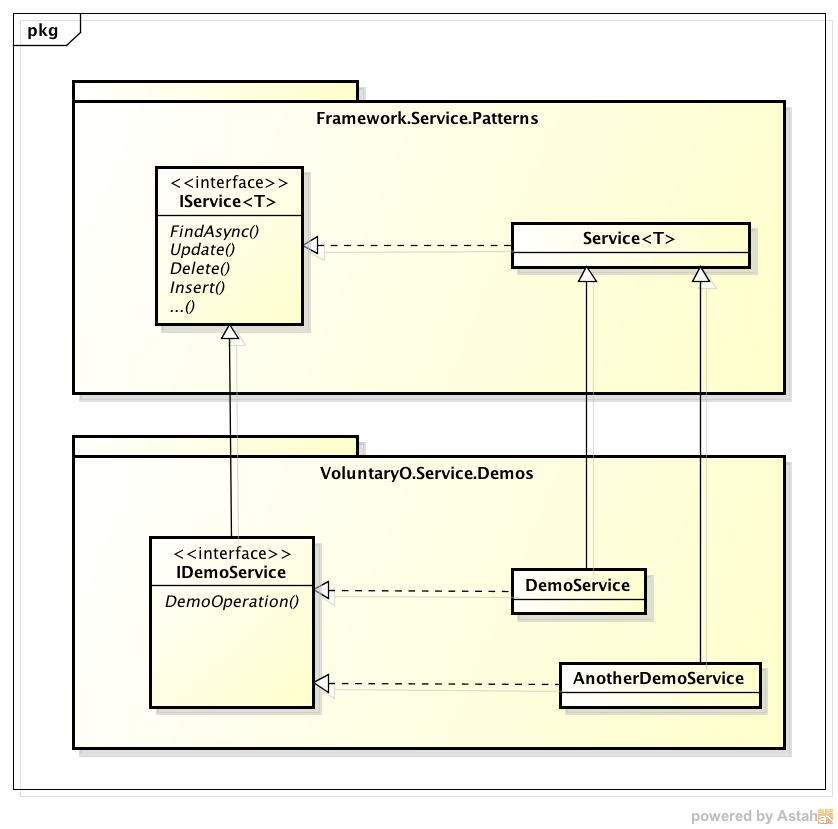
\includegraphics[width=0.9\textwidth]{content/architekturdokumentation/images/Service_Class_Hierarchy.png}
	  		\vspace{-15pt}
			\caption{Referenz-Hierarchie für Service-Klassen}
	\end{figure}
	
	Pro Repository wird ein Interface definiert (\textit{IDemoService}), welches alle spezifischen Methoden vorgibt. Jede Implementierung dieser Schnittstelle (\textit{DemoService, AnotherDemoService}) erbt zusätzlich von \textit{Service}. Der Dependency Injection Container (Unity) ist verantwortlich für die Instanziierung der richtigen Implementierung.
	
	
	\subsection{Service-Klassen im Überblick}
	

	
	\subsubsection{MemberService}
	
	Die MemberService-Klasse funktioniert als Schnittstelle zum MemberRepository. Speziell hervorzuheben ist die \textit{ImportMember}-Methode. Sie erlaubt es, freistehende Member-Objekte (externe Members), die nicht aus dem Repository stammen, kollisionsfrei zu integrieren.
	
	\begin{table}[H]
        \tablestyle
        \tablealtcolored
        \begin{tabularx}{\textwidth}{X X}
        \tableheadcolor
            \tablehead Methode & 
            \tablehead Beschreibung \\  
        \tablebody
            bool CheckIfMemberExists(Member member) & 
            Überprüft, ob ein Mitglied mit selbem Vornamen, Nachnamen und Geburtsdatum existiert. Falls nicht, wird davon ausgegangen, dass diese Person noch nicht im System vorhanden ist.  \tabularnewline
            
            bool CheckIfMemberWasModified(Member member) &
            Überprüft, ob das Mitglied existiert und Kontaktdaten oder Teamzugehörigkeit gewechselt haben. \tabularnewline
            
			Boolean ImportMember(Member member) &
			Versucht externe Members im System zu speichern. Dabei wird unterschieden, ob es sich um ein neues Mitglied, ein bestehendes mit abweichenden Angaben oder ein bestehendes, unverändertets Mitglied handelt. \tabularnewline      
			
			bool ImportMember(Member member, bool overwriteIfModified) &
			Importiert externe Members und überschreibt bestehende Member-Objekte, falls das \textit{overwriteIfModified}-Flag gesetzt wurde. \tabularnewline
            
			void UpdateMember(Member member)  &
			Aktualisiert Kontaktdaten und Teamzugehörigkeit eines Mitglieds. \tabularnewline
			
			void AssignMemberAndTeamWithInsert(Member member, string teamName) &
			Weist dem Mitglied ein echtes Team-Objekt aus dem Repository zu oder erstellt ein solches anhand des übergebenen Strings, falls es noch nicht existiert. \tabularnewline
			
			ICollection<Member> UnmodifiedRecords() &
			Externe Members, die beim Importieren übersprungen wurden, weil sie nicht verändert wurden. \tabularnewline
			
			ICollection<Member> ModifiedRecords() &
			Externe Members, die verändert und deshalb nicht abgespeichert wurden. \tabularnewline
			
			ICollection<Member> NewRecords() &
			Externe Members, die zuvor noch nicht im System vorhanden waren und abgespeichert wurden. \tabularnewline
			
				
			         
        \tableend
        
        \end{tabularx} 
    \end{table}
	
	
	\subsection{EventService}
		Der EventService verbindet den EventController mit dem Event- und HelperTaskRepository. Die Logik zum Verwalten der Relationen zwischen Helfereinsätzen, Events Mannschaften wurde hier implementiert.
		
		\begin{table}[H]
        \tablestyle
        \tablealtcolored
        \begin{tabularx}{\textwidth}{X X}
        \tableheadcolor
            \tablehead Methode & 
            \tablehead Beschreibung \\  
        \tablebody
            void AssignEventAndTeam(int eventId, int teamId) & 
            Fragt Event und Team anhand von Id's aus den Repositories ab und stellt die Relation her.  \tabularnewline
            
            void UnassignEventAndTeam(int eventId, int teamId) & 
            Fragt Event und Team anhand von Id's aus den Repositories ab und hebt die Relation auf.  \tabularnewline
            
           void InsertHelperTask(HelperTask task, int taskType, int eventId) &
           Selektiert Event- und HelperTask-Objekte, um dem Event einen Helfereinsatz zuzuordnen. \tabularnewline
           
           void DeleteHelperTask(int helperTaskId) &
           Löscht den Helfereinsatz anhand der Id. Das Event wird dazu nicht benötigt. \tabularnewline
           
           void UnassignEventAndAllTeams(Event e) &
           Entfernt alle Teams eines Events. \tabularnewline
           
           void	UnassignEventAndAllHelperTasks(Event e) &
           Entfernt alle Helfereinsätze eines Events. \tabularnewline
           
           void AssignEventAndTeam(Event e, Team team) &
           Ordnet dem Event ein weiteres zuständiges Team zu. \tabularnewline
           
           void AssignEventAndHelperTask(Event e, int helperTaskId) &
           Ordnet dem Event einen weiteren Helfereinsatz zu. \tabularnewline
           
           bool Contains(Event e) &
           Überprüft, ob ein Event bereits im Repository existiert. \tabularnewline
			
				
			         
        \tableend
        
        \end{tabularx} 
    \end{table}
	
	\subsection{TeamService}
		Bietet Zugriff auf die Methoden des TeamRepository und stellt Erweiterungspunkt für komplexere Logik dar. Diese Klasse wird im \textit{EventController} verwendet.
		
		\begin{table}[H]
        \tablestyle
        \tablealtcolored
        \begin{tabularx}{\textwidth}{X X}
        \tableheadcolor
            \tablehead Methode & 
            \tablehead Beschreibung \\  
        \tablebody
            IEnumerable<Team> GetAllTeams() & 
            Selektiert alle Teams aus dem Repository.  \tabularnewline
            
            Team GetTeamById(int id) &
            Selektiert Team aus Repository anhand der Id. \tabularnewline
	
			         
        \tableend
        
        \end{tabularx} 
    \end{table}
		
	
	\subsection{SkillService}
		Bietet Zugriff auf die Methoden des SkillRepository und stellt Erweiterungspunkt für komplexere Logik dar.
		
		\begin{table}[H]
        \tablestyle
        \tablealtcolored
        \begin{tabularx}{\textwidth}{X X}
        \tableheadcolor
            \tablehead Methode & 
            \tablehead Beschreibung \\  
        \tablebody
            public IEnumerable<Skill> GetAllSkills() & 
            Selektiert alle Skills aus dem Repository.  \tabularnewline
	
			         
        \tableend
        
        \end{tabularx} 
    \end{table}
	
	\subsection{HelperTaskService}
		Die HelferTaskService-Klasse wird von mehreren Controllern verwendet. Sie enthält wichtige Business-Logik zum An- und Abmelden für einen Helfereinsatz und prüft dazu folgende Bedingungen:
		\\\begin{itemize}
			\item Helfereinsatz ist noch nicht mit ausreichend vielen Mitgliedern belegt
			\item Mitglied hat sich noch nicht für diesen Helfereinsatz angemeldet
			\item Keine Zeitüberschneidung mit anderen Helfereinsätzen vorhanden
			\item Fähigkeiten für den Einsatz sind gegeben
		\end{itemize}
		
		\begin{table}[H]
        \tablestyle
        \tablealtcolored
        \begin{tabularx}{\textwidth}{X X}
        \tableheadcolor
            \tablehead Methode & 
            \tablehead Beschreibung \\  
        \tablebody
           void SubmitForTask(Member member, HelperTask task) & 
           Versucht, das Mitglied für einen Helfereinsatz zu registrieren. Dazu müssen alle oben genannten Bedinungen erfüllt sein. \tabularnewline
           
           void RemoveFromTask(Member member, HelperTask task) &
           Meldet das Mitglied wieder vom Helfereinsatz ab. \tabularnewline
           
           void UnassignAllMembers(HelperTask helperTask) &
           Meldet alle Mitglieder eines Helfereinsatzes ab. \tabularnewline
           
           
	
		\tableend
        
        \end{tabularx} 
    \end{table}
	
	\subsection{Imports}
		Für das Importieren von Mitgliedern und Events wird jeweils eine eigene Serviceklasse verwendet. Die abstrakte Klasse \textit{Importer} dient dazu als Basis und schreibt die Methode \textit{executeImport} vor.
		
	    \begin{figure}[h]
	  		\vspace{-5pt}
	    	\centering
	    	 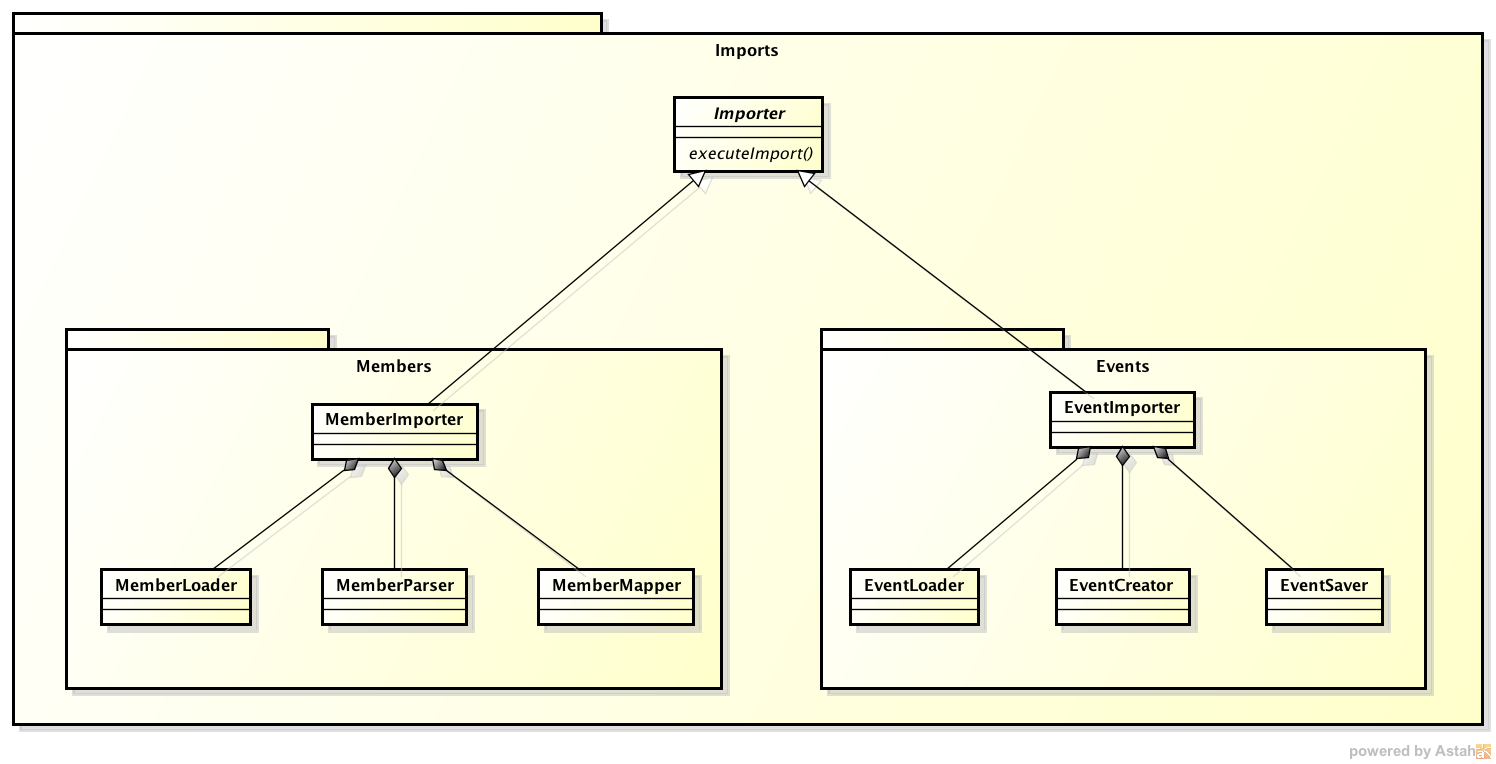
\includegraphics[width=0.9\textwidth]{content/architekturdokumentation/images/ImportPackageDesign.png}
	  		\vspace{-25pt}
			\caption{Importer-Klassen und deren direkte Collaborators}
		\end{figure}
		
		\subsubsection{MemberImporter}
			Der MemberImporter implementiert die Methode \textit{executeImport}, welche das importieren von Mitgliedern startet. Um eine höhere Kohäsion und niedrige Kopplung zu erreichen, wurden die Teilaufgaben ausgelagert:
			\\\begin{itemize}	
				\item MemberLoader - benutzt die webling.ch Schnittstelle und lädt das CSV
				\item MemberParser - liest den CSV-String und speichert die Werte in eine Liste von Hashtables
				\item MemberMapper - gibt Member-Objekte an MemberService zum Speichern weiter\\
			\end{itemize}



		\subsubsection{EventImporter}
			Der EventImporter implementiert ebenfalls die von der abstrakten Basisklasse \textit{Importer} vorgebenen Methode zum Auslösen der Import-Routine. Auch hier wurde die Arbeit in drei Teilaufgaben gegliedert:
			\\\begin{itemize}	
				\item EventLoader - lädt die Daten vom Swiss Unihockey REST Service
				\item EventCreator - liefert Liste mit Event-Objekten
				\item EventSaver - Speichet die Events in der Datenbank ab\\
			\end{itemize}
	
			\noindent
			Da Events in der Regel nur einmal pro Saison importiert werden, müssen diese nicht auf Modifikationen überprüft werden.
	
	\subsection{MailingService}
		Um das Versenden von E-Mails zu vereinfachen, kapselt diese Klasse die Vorbereitung und Konfiguration eines \textit{SmtpClient} und einer \textit{MailMessage}. Dabei werden SMTP-Host und -Port, sowie die Credentials aus dem \textit{ConfigurationManager} gelesen.  

		\begin{lstlisting}[language=CSharp, caption=Verwendung des MailingService, label=lst:mailingservice, firstnumber=1]
	var mail = new MailingService();
	mail.SendMail("nle@hsr.ch", "nle@hsr.ch", "Test Subject", "Test Message");
	    \end{lstlisting}
    



\section{VoluntaryO.Web}
	Die komplette Implementierung des Frontends befindet sich im Projekt Voluntary.Web. Folgend werden die Konzepte beschrieben, die wir zur Darstellung des Frontends verwenden.

	\subsection{Dependency Injection}
		Die Idee hinter Dependency Injection und allgemein Inversion-of-Control, ist die Anwendung des sogenannten Hollywood Prinzips: \"Don’t call us, we call you!\". 
		\\Als Dependency Injection Container wird \href{http://unity.codeplex.com/}{Unity} verwendet. Der Controller gibt in seinem Konstruktor an, welche Interfaces benötigt werden. \textit{Unity} wird diese Abhängigkeiten dann zur Laufzeit zur Verfügung stellen.
		\begin{lstlisting}[language=CSharp, caption=UnityConfig.cs, label=lst:unityconfig, firstnumber=1]
	container.RegisterType<IDataContextAsync, VoluntaryoContext>(new PerRequestLifetimeManager(), new InjectionConstructor())
	    .RegisterType<IUnitOfWork, UnitOfWork>(new PerRequestLifetimeManager())
	    .RegisterType<IUnitOfWorkAsync, UnitOfWork>(new PerRequestLifetimeManager())
	    .RegisterType<IEventRepository, EventRepository>()
	    .RegisterType<IHelperTaskRepository, HelperTaskRepository>()
	    .RegisterType<IRepository<HelperTaskType>, Repository<HelperTaskType>>()
	    .RegisterType<IMemberRepository, MemberRepository>()
	    .RegisterType<ITeamRepository, TeamRepository>()
	    .RegisterType<IRepositoryAsync<Skill>, Repository<Skill>>()
	    .RegisterType<IEventService, EventService>()
	    .RegisterType<IHelperTaskService, HelperTaskService>()
	    .RegisterType<ISkillService, SkillService>()
	    .RegisterType<IMemberService, MemberService>()
	    .RegisterType<ITeamService, TeamService>();
	    \end{lstlisting}
	    Der \textit{PerRequestLifetimeManager} hält die Instanz für den gesamten HTTP-Request. Somit erhält jeder Request ein eigener \textit{Context} und eine eigene \textit{Unit of Work}.

	\subsection{Model-View-Controller}
		Für die Presentationschicht setzen wir MVC ein, da ASP.NET eine gute Unterstützung für dieses Modell bietet. Auf alle Seiten wird mittels Controller zugegriffen. Die Views werden mithilfe der Razorsprache erstellt.

	\subsection{View Model und Razor}
		Um die Websiten dynamisch darzustellen nutzen wir die ASP.NET Razor View Engine. Eine Razor-View ist immer mit einer Methode des Controllers verbunden. Das bedeutet auch, dass der Return-Wert der Methode sämtliche Daten mitliefern muss, die später in der View gebraucht werden. Da in einer View häufig mehr als nur ein standard Objekt aus dem Model gebraucht wird, haben viele Views ein Extra Viewmodel. Das bedeutet es wird extra eine Instanz eines speziell auf die View zugeschnittenen Objekt erstellt. Dieses View-Model enthält alle Referenzen auf andere Objekte, die innerhalb der View gebraucht werden.
		Durch den Einsatz des View-Model haben wir den Vorteil, dass pro View genau definiert ist, welche Daten wir brauchen. Der Zugriff auf das View-Model kann einfach getestet werden.
		Der Einsatz eines View-Models bietet aber auch einige Nachteile, beispielsweise werden manche Methoden redundant implementiert. Da wir die Implementation der Methoden aber sowieso auf die Service-Schicht abstrahiert haben, birgt dies für uns kein Problem.
		Da wir nicht durch das Model pro View eingeschränkt werden wollen bietet uns das View-Model den besten Dienst.

	\subsection{ASP.NET Identity (Authentifizierung und Authentisierung)}
		Wir verwenden ASP.NET Identity in Version 2.0 für die Authentifizierung und Authentisierung. Folgende benutzerrelevanten Funktionen werden vom Projekt unterstützt:
		\\\begin{itemize}	
			\item Login / Logout
			\item Passwort vergessen
			\item Benutzer anlegen, importieren, bearbeiten und löschen (Admin)
			\item Rollenzuweisung
		\end{itemize}
		Diese Funktionalitäten sind im \textit{AccountController.cs} abgehandelt. Die Logik für die obigen Funktionen sind in der Klasse \textit{UserManager.cs}, welche von \textit{ASP.Net Identity} implementiert ist. Die benutzerrelevanten Funktionen sind daher Indirektionen auf den \textit{UserManager}.

		\subsubsection{Rollen}
			\begin{itemize}
				\item Member
				\item Planer
				\item Admin
			\end{itemize}
			Die Rollen werden für die Authentisierung für Controller-Actions und Views benötigt.
			\begin{lstlisting}[language=CSharp, caption=AccountController.cs, label=lst:accountcontroller, firstnumber=1]
// GET: /Acount/Edit/madminis
[Authorize(Roles = "Admin")]
public ActionResult Edit(string id, ManageMessageId? Message = null) {}
			\end{lstlisting}

			Authentisierung in View:
			\begin{lstlisting}[language=CSharp, caption=\_Layout.cshtml, label=lst:layoutauthentisierung, firstnumber=1]
@if (User.IsInRole("Admin") || User.IsInRole("Admin"))
			\end{lstlisting}

		\subsubsection{Passwortverschlüsselung}
		Das Passwort wird als Hash (\textit{HMACSHA256}) in der Datenbank abgespeichert. Das Projekt verwendet die Standardimplementation von Asp.Net Idenity mit \textit{PasswordHasher}. Der \textit{PasswordHasher} verwendet die \href{http://de.wikipedia.org/wiki/PBKDF2}{\textit{PBKDF2}} um den Hash inkl. einen Saltwert zu strecken. Die Streckung wird 5000 mal durchgeführt. Diese Verkettung erschwert es, per Brute-Force-Methode aus dem Schlüssel auf das ursprüngliche Passwort zu schliessen.


	\subsection{Bootstrap, CSS und JS}
		Das Front-End Framework, dass wir einsetzen ist Twitter Bootstrap. Zusätzlich verwenden wir ein verändertes CSS-File um nicht den typischen Bootstrap-Look zu erhalten.
		Zusätzlich setzen wir die Javascript-Library JQuery ein.
		ASP.NET bietet einen für die Einbindung von CSS- und JS-Files einen Bundle-Konfigurator an. So können CSS-Files oder JS-Files in Bundles gruppiert werden. Per View kann man dann genau definieren welche Bundles aktuell gebraucht werden. ASP.NET bindet einem dann automatisch die entsprechen Files in die HTML-Datei ein.
		Besonders nützlich ist hier, dass während der Entwicklungs-Phase die Files noch einzeln und noch nicht minifiziert übertragen werden. Sobald man die Applikation aber auf den Server deployed werden die Files automatisch in ein File gerendert und auch minifiziert, was für die Übertragungsgeschwindigkeit wichtig sein kann.
		Dabei wird pro Bundle ein File ausgeliefert, was besonders für das HTML-Caching wichtig ist.

	\subsection{AJAX und WebAPI}
		Unser Ziel ist es, dass unsere Applikation möglichst dynamisch sein soll. Dafür ist der Einsatz von asynchronen Request extrem wichtig. In unserer Applikationen sind mehrere verschiedene Implementationsarten dieses Konzeptes eingesetzt worden. Wenn möglich wurden die direkt von ASP.NET unterstützten Features genutzt. Hier wird über ein sogenanntes Ajax-Form in der Razor-Syntax ein AJAX Befehl konfiguriert. Als Return-Value wird hier ein Partial-View zurückgegeben. Dieser ersetzt dann ein bestehendes Partial-View.
		Besonders gut ist hier, dass unobstrusive-AJAX eingesetzt wird. Das bedeutet dieser Code würde auch funktionieren, wenn Javascript nicht aktiviert wäre.
		Für die komplexeren AJAX-Requests, die nicht mehr durch die ASP.NET Boardmittel gelöst werden können, haben wir ein REST Web-Api implementiert. Dieses API ermöglicht es durch AJAX-Request JSON Daten zurückzukriegen und diese dann dynamisch auf der Seite zu implementieren.
		Das Web-Api ist massgebend für die dynamik der Page.
